% Neuf services du périmètre et dernier test de restauration documenté (T09)
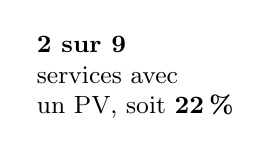
\begin{tikzpicture}[font=\scriptsize]
  \def\tiret{-}
  \foreach \sv/\dt [count=\i from 0] in \Sauvegardes{
    \pgfmathtruncatemacro\col{mod(\i,5)}\pgfmathtruncatemacro\lig{div(\i,5)}
    \ifx\dt\tiret \def\kcol{gris}\def\ktxt{aucun PV fourni}\else\def\kcol{vert}\def\ktxt{PV du \dt/2026}\fi
    \node[draw=\kcol, fill=\kcol!10, rounded corners=2pt, minimum width=2.75cm, minimum height=0.95cm, align=center]
      at (\col*2.95,-\lig*1.15) {\textbf{\sv}\\[-1pt]{\color{\kcol}\ktxt}};}
  \node[anchor=west, align=left, font=\small] at (11.95,-1.15) {\textbf{2 sur 9}\\ services avec\\ un PV, soit \textbf{22\,\%}};
\end{tikzpicture}
